% Project presentation (Beamer), about 30 minutes.  Build:  cd slides/beamer && latexmk -pdf slides.tex
% slides/make_pptx.py then turns the PDF into Project51_ManasJain.pptx (one slide image per page).
\documentclass[aspectratio=169,11pt]{beamer}
\usetheme{Madrid}
\definecolor{teal}{RGB}{0,95,100}
\usecolortheme[named=teal]{structure}
\setbeamertemplate{navigation symbols}{}
\usepackage{amsmath,amssymb}
\usepackage{booktabs}
\usepackage{graphicx}
\usepackage{tikz}
\graphicspath{{../../figures/}{./}}

% watermark: lion image in the centre of every slide, behind the content
\setbeamertemplate{background}{%
  \begin{tikzpicture}[remember picture,overlay]
    \node at (current page.center) {
\includegraphics[width=0.55\paperwidth]{lion.png}};
  \end{tikzpicture}}

\title[AI-based 3D surface area estimation]{AI-based 3D surface area estimation\\ from CT-like voxel data}
\subtitle{PHC-351 Course Project 51}
\author[Manas Jain]{Manas Jain\\[2pt] {\small Enrolment no.\ 24123021}}
\date{}

\begin{document}

% 1 ------------------------------------------------------------------
\begin{frame}
  \titlepage
\end{frame}

% 2
\begin{frame}{Outline}
  \begin{enumerate}
    \item Introduction: why surface area, what a CT scan gives us, how area is measured
    \item Problem and objectives
    \item Theory: why each classical method is wrong, and by how much
    \item Previous work
    \item Method: data, exact reference areas, models, training
    \item Live demo
    \item Results: accuracy, noise, object size, grid size, unseen shapes, failure case
    \item Conclusion, limitations and next steps
  \end{enumerate}
\end{frame}

\section{Introduction}
% 3
\begin{frame}{Why surface area matters}
  Surface area is measured from X-ray CT scans in many fields:
  \begin{itemize}
    \item \textbf{Catalysts}: reactions happen on the surface, so more area means more activity.
    \item \textbf{Filters and rocks}: the pore surface controls how fluid flows through the material.
    \item \textbf{3D-printed lattices}: the area shows whether a part matches its design.
  \end{itemize}
  \vspace{1em}
  \begin{block}{Question of this project}
    How wrong is the surface area we measure from a CT scan, and can a learned model correct it?
  \end{block}
\end{frame}

% 4
\begin{frame}{What a CT scan gives us}
  \begin{columns}[T]
    \begin{column}{0.48\textwidth}
      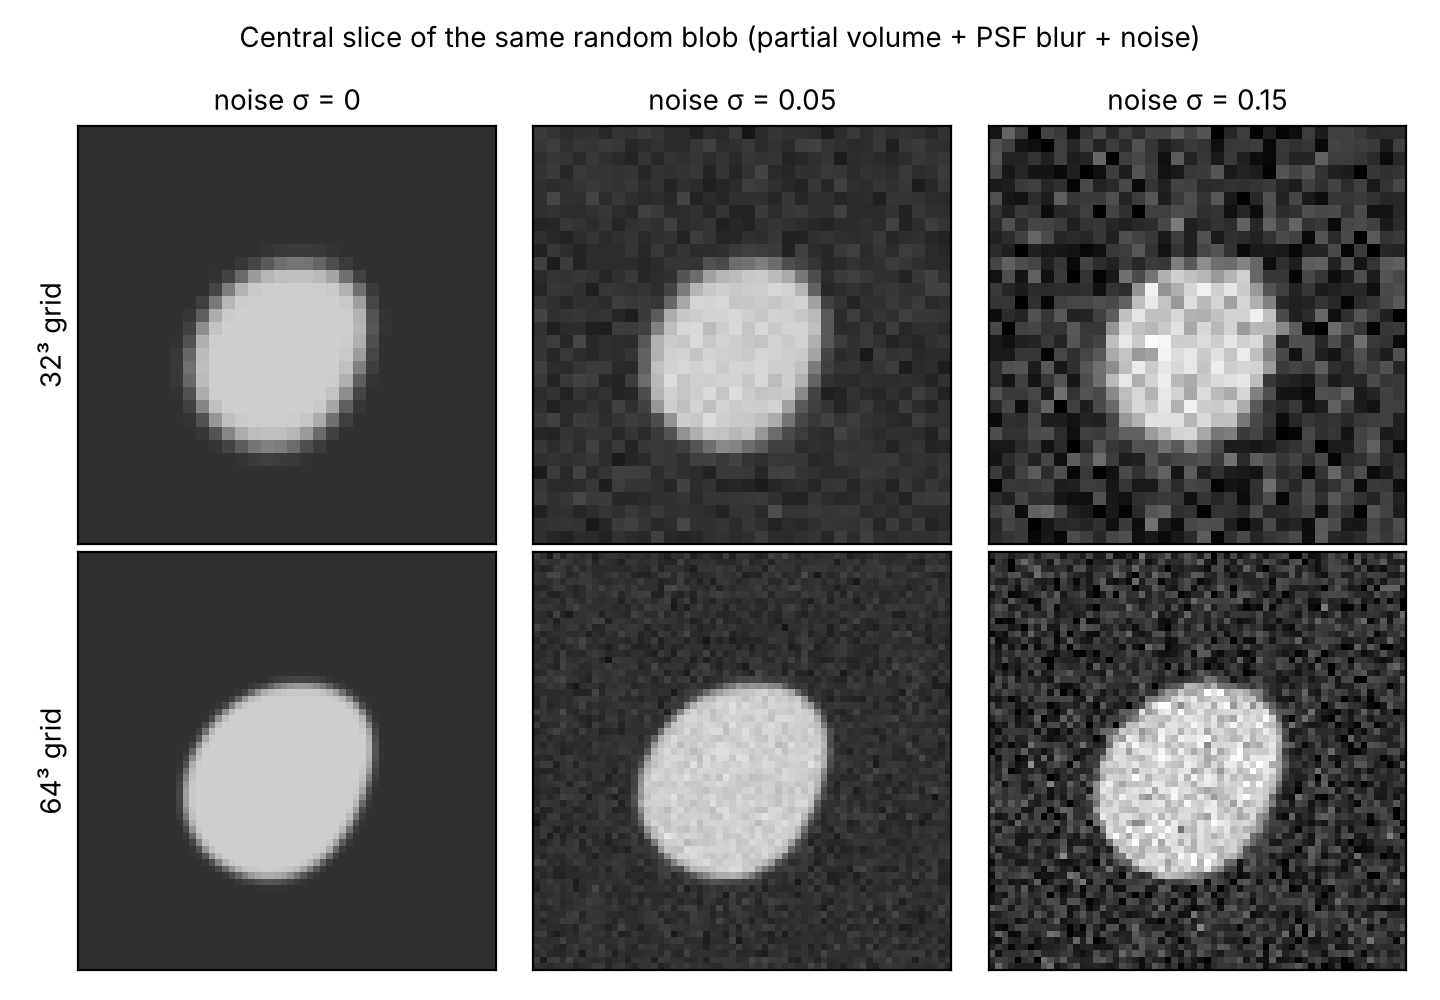
\includegraphics[width=\linewidth]{example_slices.png}
      {\scriptsize Same blob at $32^3$ and $64^3$, noise $\sigma_n = 0,\ 0.05,\ 0.15$.}
    \end{column}
    \begin{column}{0.5\textwidth}
      \begin{itemize}
        \item A 3D grid of small cubes (\textbf{voxels}).
        \item Each voxel stores one grey value: dark outside, bright inside.
        \item No surface is stored anywhere: it has to be reconstructed.
      \end{itemize}
    \end{column}
  \end{columns}
\end{frame}

% 5
\begin{frame}{Three things that blur the picture}
  \begin{enumerate}
    \item \textbf{Partial volume}: a voxel's value is the fraction of it inside the object.
          \[ v = \frac{\text{volume of voxel inside the object}}{\text{volume of voxel}} \]
          A voxel half inside comes out half grey.
    \item \textbf{Scanner blur} (point-spread function): each value is mixed with its neighbours.
    \item \textbf{Noise}: random fluctuations added to every voxel.
  \end{enumerate}
  \vspace{0.5em}
  \begin{block}{Consequence}
    The surface lies between voxel centres. Every method that reconstructs it adds some error.
  \end{block}
\end{frame}

% 6
\begin{frame}{Two standard ways to measure area}
  \centering
  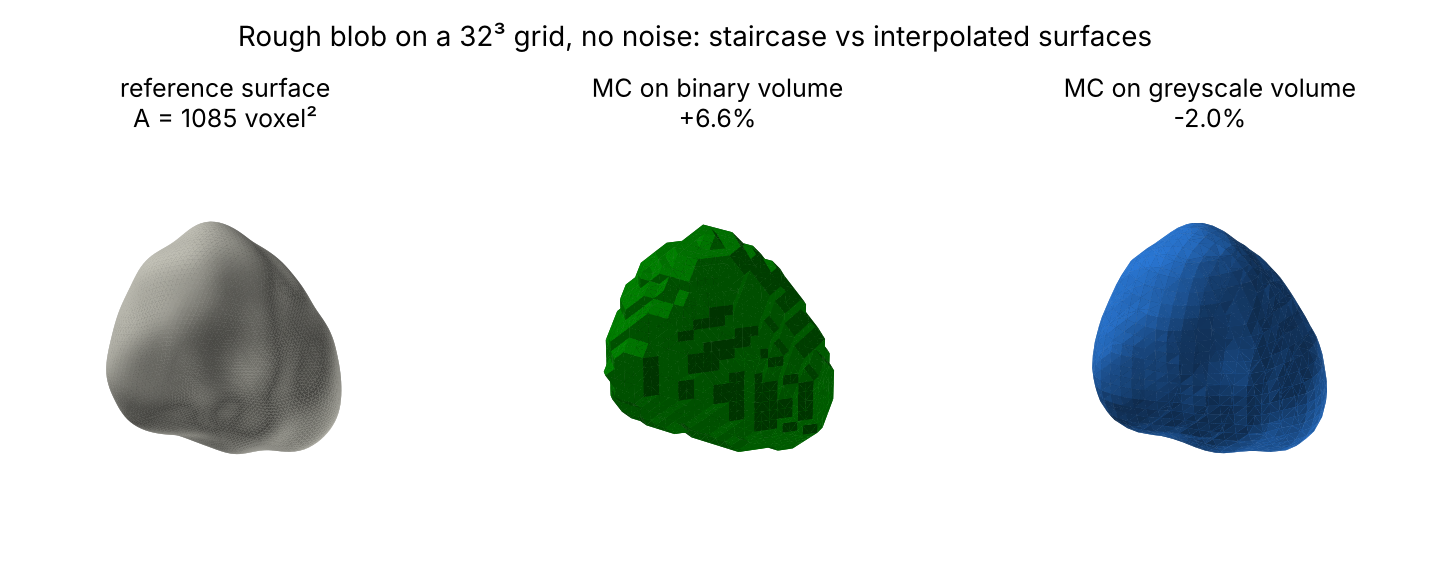
\includegraphics[width=0.78\textwidth]{example_meshes.png}
  \vspace{0.3em}
  \begin{columns}[T]
    \begin{column}{0.46\textwidth}
      \textbf{1. Count voxel faces}\\
      \small Threshold at 0.5, count the faces on the outside of the inside voxels.
    \end{column}
    \begin{column}{0.46\textwidth}
      \textbf{2. Marching cubes}\\
      \small Fit a triangle mesh through the grid and add up the triangle areas.
    \end{column}
  \end{columns}
\end{frame}

% 7
\begin{frame}{How marching cubes works}
  \begin{itemize}
    \item Look at each $2\times2\times2$ cell of voxels.
    \item Wherever the value crosses the iso-level 0.5 along an edge, place a vertex.
    \item Connect the vertices into triangles using a lookup table of cell patterns.
  \end{itemize}
  \vspace{0.5em}
  Where on the edge? Between voxels with values $v_a$ and $v_b$:
  \[ t = \frac{0.5 - v_a}{v_b - v_a} \]
  \begin{columns}[T]
    \begin{column}{0.46\textwidth}
      \begin{block}{Binary volume}
        Values are 0 or 1, so $t = 0.5$ always: vertices only at edge midpoints.
      \end{block}
    \end{column}
    \begin{column}{0.46\textwidth}
      \begin{block}{Greyscale volume}
        $t$ can take any value, so the surface can sit anywhere between voxels.
      \end{block}
    \end{column}
  \end{columns}
\end{frame}

% 8
\begin{frame}{Problem and objectives}
  \begin{block}{Problem}
    Given a blurred, noisy voxel volume of one object, estimate the area of its true surface.
  \end{block}
  \textbf{Objectives}
  \begin{enumerate}
    \item Shapes with a true area known to better than 1 part in 10{,}000.
    \item Measure the error of voxel faces and three marching-cubes variants.
    \item Learn a correction (3D CNN, PointNet, Random Forest) and compare it with a lookup table.
    \item Test on shape families never seen in training.
    \item Say when a learned correction is worth using.
  \end{enumerate}
\end{frame}

\section{Theory}
% 9
\begin{frame}{Theory 1: why voxel faces measure a staircase}
  \begin{columns}[T]
    \begin{column}{0.55\textwidth}
      \begin{itemize}
        \item A flat patch of area $A$ with unit normal $\mathbf n = (n_x, n_y, n_z)$.
        \item Its voxel version is a staircase of faces pointing along $x$, $y$ and $z$.
        \item The $x$-faces add up to the shadow of the patch on the $yz$ plane: $A\,|n_x|$.
        \item Same for $y$ and $z$, so
      \end{itemize}
      \[ \frac{A_\text{faces}}{A} = r(\mathbf n) = |n_x| + |n_y| + |n_z| \]
    \end{column}
    \begin{column}{0.4\textwidth}
      \begin{block}{Range}
        $r = 1$ only when the patch is aligned with the grid.\\[3pt]
        $r = \sqrt3 \approx 1.73$ on the main diagonal.
      \end{block}
    \end{column}
  \end{columns}
\end{frame}

% 10
\begin{frame}{Theory 1: on average 50\% too high, at any resolution}
  \begin{columns}[T]
    \begin{column}{0.5\textwidth}
      \begin{itemize}
        \item For random orientations, each $|n_i|$ is uniform on $[0,1]$, so $\langle|n_i|\rangle = 1/2$.
        \item Therefore $\langle r\rangle = 3/2$: a $+50\%$ error.
        \item $r$ does not contain the voxel size: smaller voxels give finer steps, not flatter ones.
      \end{itemize}
      \vspace{0.5em}
      \begin{block}{Measured, clean sphere at $128^3$}
        Voxel faces: $+50.0\%$
      \end{block}
    \end{column}
    \begin{column}{0.46\textwidth}
      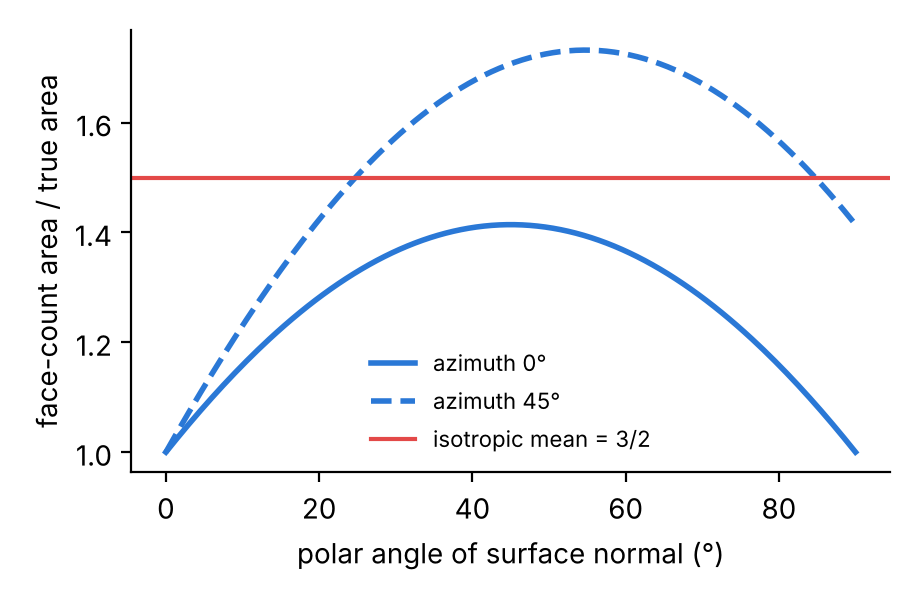
\includegraphics[width=\linewidth]{face_count_theory.png}
    \end{column}
  \end{columns}
\end{frame}

% 11
\begin{frame}{Theory 2: binary marching cubes never converges}
  \begin{itemize}
    \item On a binary volume every vertex is at an edge midpoint.
    \item So only a few triangle orientations are possible, and a tilted plane becomes a fine
          zig-zag with extra area.
    \item Smaller voxels make the zig-zag finer but not flatter (Kenmochi and Klette 2000).
  \end{itemize}
  \vspace{0.5em}
  \centering
  \begin{tabular}{lrrrr}
    \toprule
    Clean spheres & $16^3$ & $32^3$ & $64^3$ & $128^3$ \\
    \midrule
    Voxel faces & $+49.0\%$ & $+49.1\%$ & $+49.7\%$ & $+50.0\%$ \\
    Binary MC & $+7.3\%$ & $+8.1\%$ & $+8.6\%$ & $+8.8\%$ \\
    \bottomrule
  \end{tabular}
  \vspace{0.3em}

  Both errors stay put as the grid is refined; the binary one even grows slightly.
\end{frame}

% 12
\begin{frame}{Theory 3: greyscale marching cubes and curvature}
  \begin{itemize}
    \item Greyscale values let the vertices sit between voxels. For a flat surface and a symmetric
          blur, the 0.5 level lies exactly on the true surface.
    \item For a curved surface it does not. Blurring spreads the object's brightness outwards
          over a larger volume, so the half-brightness surface sits slightly \textbf{inside} the
          true one.
    \item The more sharply the surface bends, the bigger the shift.
  \end{itemize}
  \vspace{0.5em}
  \begin{alertblock}{Result}
    Greyscale marching cubes is slightly too small on curved surfaces, especially for small objects.
  \end{alertblock}
\end{frame}

% 13
\begin{frame}{Theory 3: a prediction we can test}
  \begin{columns}[T]
    \begin{column}{0.5\textwidth}
      Gaussian blur is diffusion, so the 0.5 level moves inwards by
      \[ \delta \approx \sigma^2 H, \qquad H = \text{mean curvature}. \]
      For a sphere of radius $R$, $H = 1/R$, and
      \[ \frac{\Delta A}{A} \approx -\frac{2\sigma^2}{R^2}. \]
      Our blur: voxel box $1/12$ + scanner $0.6^2$ gives $\sigma^2 \approx 0.44$ voxel$^2$.
    \end{column}
    \begin{column}{0.46\textwidth}
      \centering\small
      Clean spheres, greyscale MC\\[4pt]
      \begin{tabular}{rrrr}
        \toprule
        Grid & $R$ & Predicted & Measured \\
        \midrule
        $16^3$  & 5.4  & $-3.04\%$ & $-3.65\%$ \\
        $32^3$  & 12.6 & $-0.56\%$ & $-0.62\%$ \\
        $64^3$  & 27.0 & $-0.12\%$ & $-0.05\%$ \\
        $128^3$ & 55.8 & $-0.03\%$ & $+0.07\%$ \\
        \bottomrule
      \end{tabular}
    \end{column}
  \end{columns}
\end{frame}

% 14
\begin{frame}{Theory 4: noise creates fake specks}
  \begin{itemize}
    \item A background voxel crosses the 0.5 threshold by chance with probability
          \[ p = Q\!\left(\frac{0.5}{\sigma_n}\right) \quad (Q = \text{Gaussian tail}). \]
    \item At $\sigma_n = 0.15$: $p \approx 4.3\times10^{-4}$, so about \textbf{112 specks} on a
          $64^3$ grid and 14 on a $32^3$ grid.
    \item Each speck is a tiny closed surface that adds area.
    \item The Euler number (number of separate pieces, roughly) counts them: we measure about
          100 to 125 at $64^3$.
    \item At $\sigma_n = 0.05$: $p = Q(10)$, effectively zero.
  \end{itemize}
\end{frame}

% 15
\begin{frame}{Theory 4: rough surfaces, and why smoothing is no cure}
  \begin{itemize}
    \item Noise also roughens the real surface, and a rough surface always has more area than a
          smooth one.
    \item Smoothing the volume first removes most of the noise, but:
          \begin{itemize}
            \item it increases the blur ($\sigma^2$ from 0.44 to 1.44), so the curvature error
                  grows about $3\times$;
            \item it erases structures thinner than about two voxels completely.
          \end{itemize}
  \end{itemize}
  \vspace{0.5em}
  \centering
  \begin{tabular}{lrr}
    \toprule
    MC after smoothing, test MAPE & $32^3$ & $64^3$ \\
    \midrule
    All shapes & 13.78\% & 3.04\% \\
    \bottomrule
  \end{tabular}
\end{frame}

% 16
\begin{frame}{Theory: two errors pulling in opposite directions}
  \begin{columns}[T]
    \begin{column}{0.46\textwidth}
      \begin{block}{Curvature: area too small}
        Strongest for small objects and coarse grids.
      \end{block}
    \end{column}
    \begin{column}{0.46\textwidth}
      \begin{block}{Noise: area too big}
        Strongest for noisy scans and fine grids.
      \end{block}
    \end{column}
  \end{columns}
  \vspace{1em}
  \begin{alertblock}{Consequence}
    The size of each effect depends on the object and the scan, so no single correction factor can
    fix both. The correction has to be worked out object by object, which is what a learned model
    can do.
  \end{alertblock}
\end{frame}

\section{Previous work}
% 17
\begin{frame}{Previous work 1: digital geometry}
  \begin{itemize}
    \item \textbf{Mesh vs voxels}: triangulated surfaces are much more accurate than voxel-face
          surfaces (Nystr\"om et al.\ 2002).
    \item \textbf{Better fixed weights}: optimal weights for each local $2\times2\times2$ voxel
          pattern (Mullikin and Verbeek 1993; Windreich et al.\ 2003; Lindblad 2005).
    \item \textbf{Convergence}:
          \begin{itemize}
            \item binary marching cubes does not converge to the true area, even for spheres
                  (Kenmochi and Klette 2000);
            \item no local estimator converges on convex polytopes (Svane 2013).
          \end{itemize}
  \end{itemize}
  \vspace{0.5em}
  These results explain the fixed errors of the binary methods, and point towards using greyscale
  information.
\end{frame}

% 18
\begin{frame}{Previous work 2: learning on 3D data, and the gap}
  \begin{itemize}
    \item 3D CNNs on voxel grids (VoxNet, 2015) and PointNet on point sets (2017) are standard
          tools for 3D shape analysis.
    \item DeePore (2020): a CNN predicts properties of porous media from micro-CT images, but
          without an exact ground truth for surface area.
    \item Random Forests on hand-picked features remain a strong baseline for small problems.
  \end{itemize}
  \vspace{0.5em}
  \begin{block}{Gap addressed here}
    Measure, against an exact reference, how much a learned model really reduces the error of
    marching cubes, separately by resolution, noise and unseen shape family, and compare it with a
    simple baseline.
  \end{block}
\end{frame}

\section{Method}
% 19
\begin{frame}{Method: seven shape families}
  \centering\small
  \begin{tabular}{llrl}
    \toprule
    Family & Role & Shapes & Parameters \\
    \midrule
    Sphere & train & 150 & radius 1 \\
    Ellipsoid & train & 350 & axes $1$, $b, c \in [0.35, 1]$ \\
    Cylinder (capped) & train & 300 & radius $0.3$ to $0.85$ \\
    Torus & train & 300 & tube/ring ratio $0.2$ to $0.6$ \\
    Smooth blob & train & 900 & 6 low-frequency waves on a sphere \\
    \midrule
    Superellipsoid & held out & 200 & pointed tips or box-like rounded edges \\
    Rough blob & held out & 200 & smooth blob + 10 high-frequency waves \\
    \bottomrule
  \end{tabular}
  \vspace{0.6em}

  \raggedright
  The two held-out families have features the training shapes never have: sharp edges and
  fine roughness.
\end{frame}

% 20
\begin{frame}{Method: making CT-like volumes}
  \begin{columns}[T]
    \begin{column}{0.52\textwidth}
      \begin{enumerate}
        \item Scale (diameter 9.8 to 60 voxels), rotate randomly, shift by a sub-voxel offset.
        \item \textbf{Partial volume}: $5\times5\times5$ samples per voxel near the surface.
        \item \textbf{Blur}: Gaussian, $\sigma = 0.6$ voxel.
        \item \textbf{Noise}: Gaussian, $\sigma_n \in \{0, 0.05, 0.15\}$.
        \item Store as 8-bit values.
      \end{enumerate}
      Every shape at $32^3$ and $64^3$ and all three noise levels: 6 volumes per shape.
    \end{column}
    \begin{column}{0.44\textwidth}
      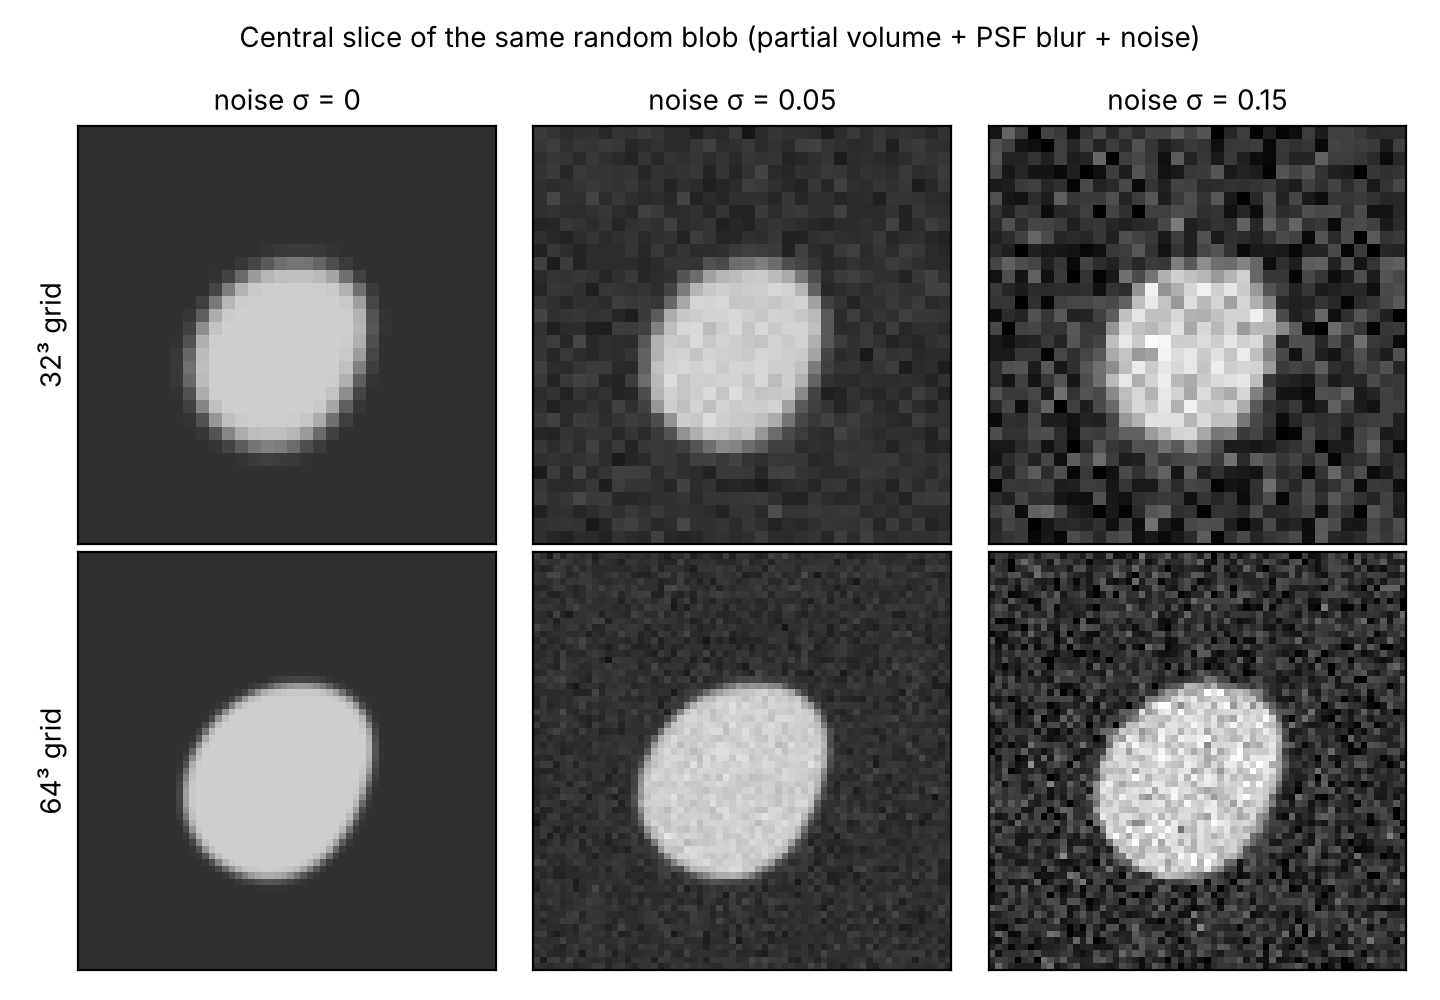
\includegraphics[width=\linewidth]{example_slices.png}
    \end{column}
  \end{columns}
\end{frame}

% 21
\begin{frame}{Method: the exact reference area}
  \begin{itemize}
    \item \textbf{Exact formulas}: sphere, cylinder, torus, and ellipsoid (using elliptic integrals).
    \item \textbf{Blobs and superellipsoids}: a very fine triangle mesh at two levels of detail
          ($81{,}920$ and $327{,}680$ triangles), combined to cancel the main error:
          \[ A_\text{ref} = \tfrac13\,(4A_\text{fine} - A_\text{coarse}) \]
    \item Remaining error below $0.01\%$ for every shape; 14 of 14 checks pass.
  \end{itemize}
  \vspace{0.5em}
  \begin{alertblock}{Why not marching cubes on a very fine grid?}
    Binary marching cubes never converges, so it would put its own error into the ground truth.
  \end{alertblock}
\end{frame}

% 22
\begin{frame}{Method: the dataset}
  \begin{columns}[T]
    \begin{column}{0.5\textwidth}
      \centering
      \begin{tabular}{rl}
        \toprule
        2{,}400 & shapes \\
        14{,}400 & CT-like volumes \\
        1{,}400 & training shapes \\
        299 & validation shapes \\
        301 & test shapes \\
        400 & held-out shapes (2 families) \\
        \bottomrule
      \end{tabular}
    \end{column}
    \begin{column}{0.46\textwidth}
      \begin{itemize}
        \item Split \textbf{by shape}, 70/15/15 within each training family, so all six
              volumes of a shape stay together.
        \item No shape appears in both training and testing.
        \item Fixed random seed (51): the whole dataset can be regenerated exactly.
      \end{itemize}
    \end{column}
  \end{columns}
\end{frame}

% 23
\begin{frame}{Method: what the models learn}
  The models do not predict the area directly. They predict a \textbf{correction} to the greyscale
  marching-cubes area:
  \[ y = \log \frac{A_\text{true}}{A_\text{MC}}, \qquad \hat A = A_\text{MC}\, e^{\hat y} \]
  \begin{itemize}
    \item Marching cubes is already close, so the model only has to learn the small remaining error.
    \item $y$ does not depend on the object's size or orientation.
    \item So each training volume can be rotated and flipped into \textbf{48 versions} (the
          symmetries of a cube) without changing the true area.
  \end{itemize}
\end{frame}

% 24
\begin{frame}{Method: the baselines}
  \begin{block}{Lookup table}
    One fixed correction per resolution and noise level (the median from training). It is even
    given the true noise level. A learned model must beat it to show it does more than apply an
    average.
  \end{block}
  \begin{block}{Random Forest (400 trees) on 10 simple measurements}
    Marching-cubes area relative to the grid; ratios of the face, binary and smoothed areas to it;
    compactness; two aspect ratios; Euler number; noise estimate; grid size $N$.
  \end{block}
\end{frame}

% 25
\begin{frame}{Method: the 3D CNN}
  \begin{columns}[T]
    \begin{column}{0.55\textwidth}
      \begin{itemize}
        \item Input: the whole $N^3$ greyscale volume.
        \item 5 convolution blocks with 16, 32, 64, 128 and 256 channels ($3^3$ kernels, batch
              norm, ReLU, max pooling).
        \item Global average and max pooling, so the same network works at $32^3$ and $64^3$.
        \item A small head (128 units) outputs $\hat y$.
        \item 3.59 million parameters.
      \end{itemize}
    \end{column}
    \begin{column}{0.4\textwidth}
      \begin{block}{Why a CNN?}
        It can see everything at once: object size, curvature, thin parts and noise specks.
      \end{block}
    \end{column}
  \end{columns}
\end{frame}

% 26
\begin{frame}{Method: PointNet}
  \begin{columns}[T]
    \begin{column}{0.55\textwidth}
      \begin{itemize}
        \item Input: 2{,}048 points sampled on the greyscale marching-cubes surface.
        \item A shared network maps each point to 1{,}024 features; max pooling combines them.
        \item A small head (512, 128 units) outputs $\hat y$.
        \item Random rotations during training instead of an alignment network.
        \item 0.74 million parameters.
      \end{itemize}
    \end{column}
    \begin{column}{0.4\textwidth}
      \begin{block}{Why test it?}
        A point cloud is a natural description of a surface, and much smaller than a volume.
      \end{block}
    \end{column}
  \end{columns}
\end{frame}

% 27
\begin{frame}{Method: training}
  \begin{columns}[T]
    \begin{column}{0.5\textwidth}
      \begin{itemize}
        \item One model per grid size.
        \item Huber loss on $y/0.05$ (quadratic below a 5\% error).
        \item AdamW, one-cycle learning rate (peak $10^{-3}$), batch 32.
        \item Up to 40 epochs; 15 for the $64^3$ CNN.
        \item Early stopping on the validation error.
        \item Apple-silicon laptop: about 60 s per epoch at $32^3$, 7 min at $64^3$.
      \end{itemize}
    \end{column}
    \begin{column}{0.46\textwidth}
      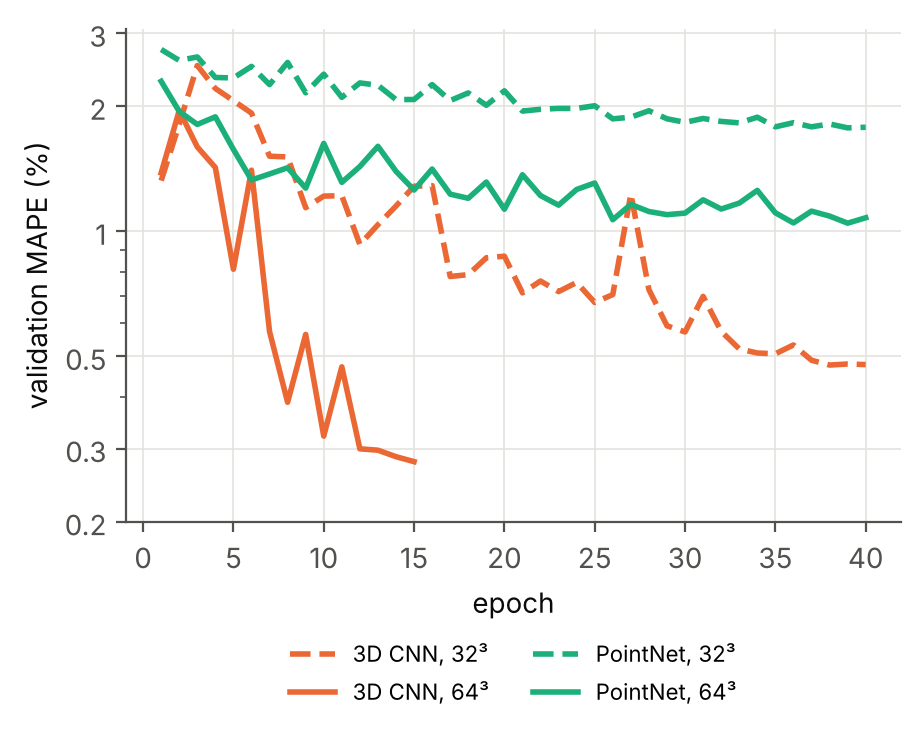
\includegraphics[width=\linewidth]{training_curves.png}
    \end{column}
  \end{columns}
\end{frame}

\section{Demo}
% 28
\begin{frame}[fragile]{Live demo}
  \footnotesize
\begin{verbatim}
$ python src/demo.py --example blob --N 64 --noise 0.15
synthetic blob, 64^3 grid, noise 0.15, diameter 55.7 voxels
Voxel-face counting          +83.72%
Marching cubes (binary)      +23.37%
Marching cubes (greyscale)    +9.25%
3D CNN correction             +0.24%

$ python src/demo.py --example ellipsoid --N 32 --noise 0.05
synthetic ellipsoid, 32^3 grid, noise 0.05, diameter 10.5 voxels
Marching cubes (greyscale)    -7.52%
3D CNN correction             -0.96%
\end{verbatim}
  \normalsize
  Noise pushes greyscale MC up, curvature pulls it down; the same CNN corrects both.
\end{frame}

\section{Results}
% 29
\begin{frame}{Results: test shapes never seen in training}
  \begin{columns}[T]
    \begin{column}{0.5\textwidth}
      \centering
      \begin{tabular}{lrr}
        \toprule
        Average error (MAPE) & $32^3$ & $64^3$ \\
        \midrule
        Voxel faces & 56.71\% & 65.54\% \\
        MC (binary) & 10.38\% & 14.49\% \\
        MC (greyscale) & 4.78\% & 3.52\% \\
        MC (smoothed) & 13.78\% & 3.04\% \\
        \midrule
        MC + lookup & 2.97\% & 0.79\% \\
        PointNet & 1.98\% & 1.04\% \\
        Random Forest & 0.72\% & \textbf{0.18\%} \\
        3D CNN & \textbf{0.68\%} & 0.26\% \\
        \bottomrule
      \end{tabular}
    \end{column}
    \begin{column}{0.46\textwidth}
      \begin{itemize}
        \item The CNN cuts the greyscale MC error 7 to 13 times.
        \item Its average bias is within $\pm0.1\%$.
        \item The Random Forest does just as well, and best at $64^3$.
        \item PointNet is clearly weaker.
      \end{itemize}
    \end{column}
  \end{columns}
\end{frame}

% 30
\begin{frame}{Results: what the Random Forest learned}
  \begin{columns}[T]
    \begin{column}{0.48\textwidth}
      \centering
      \begin{tabular}{lr}
        \toprule
        Measurement & Importance \\
        \midrule
        Euler number (counts specks) & 0.29 \\
        Noise estimate & 0.26 \\
        Smoothed / raw MC area & 0.22 \\
        Faces / MC area & 0.08 \\
        Everything else & 0.15 \\
        \bottomrule
      \end{tabular}
    \end{column}
    \begin{column}{0.48\textwidth}
      \begin{itemize}
        \item The top two measure exactly the two noise effects from the theory.
        \item The smoothed-to-raw ratio measures how much the surface responds to smoothing: a
              stand-in for curvature and thin parts.
        \item Physics-based features carry most of the information.
      \end{itemize}
    \end{column}
  \end{columns}
\end{frame}

% 31
\begin{frame}{Results: robust to noise}
  \centering
  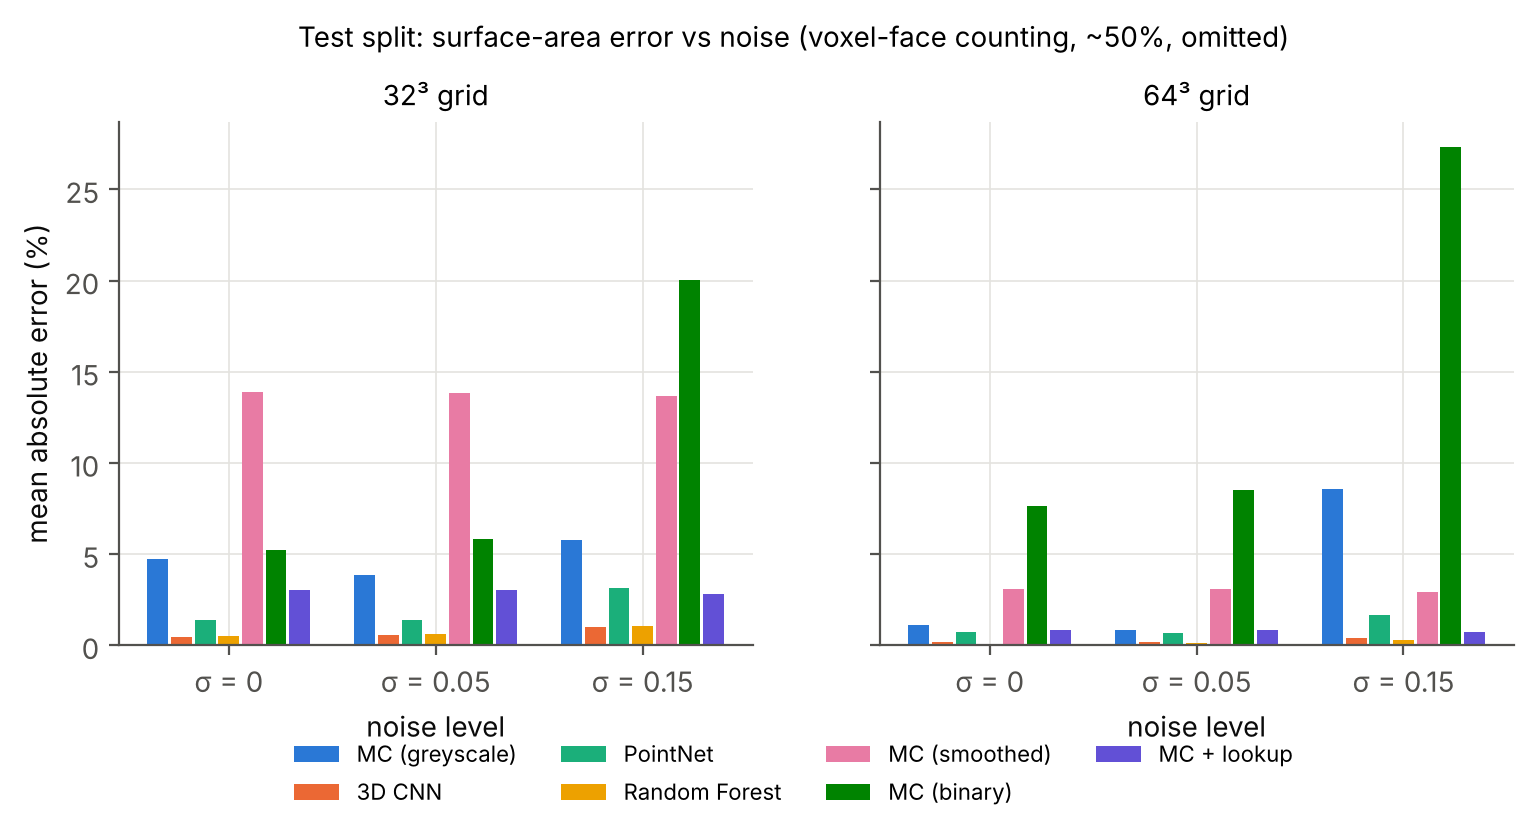
\includegraphics[width=0.7\textwidth]{error_vs_noise.png}
  \begin{itemize}
    \item $64^3$: greyscale MC goes from 1.13\% (clean) to 8.56\% (highest noise).
    \item The CNN only goes from 0.20\% to 0.40\%; the Random Forest from 0.09\% to 0.30\%.
  \end{itemize}
\end{frame}

% 32
\begin{frame}{Results: object size matters more than grid size}
  \centering
  \begin{tabular}{lrrrrr}
    \toprule
    Object diameter (voxels) & $<16$ & 16--24 & 24--32 & 32--48 & 48--64 \\
    \midrule
    MC (greyscale) & 6.43\% & 3.89\% & 3.57\% & 3.45\% & 3.44\% \\
    MC + lookup & 4.76\% & 1.78\% & 1.48\% & 0.67\% & 0.58\% \\
    Random Forest & 1.41\% & \textbf{0.39\%} & \textbf{0.22\%} & \textbf{0.13\%} & \textbf{0.08\%} \\
    PointNet & 2.14\% & 1.57\% & 1.54\% & 0.81\% & 1.48\% \\
    3D CNN & \textbf{1.24\%} & \textbf{0.39\%} & 0.28\% & 0.22\% & 0.22\% \\
    \bottomrule
  \end{tabular}
  \vspace{0.8em}
  \begin{itemize}
    \item Small objects: the CNN is best; this is where seeing the whole image pays off.
    \item Large objects: the Random Forest is best, down to 0.08\%.
  \end{itemize}
\end{frame}

% 33
\begin{frame}{Results: the theory holds across grid sizes}
  \centering
  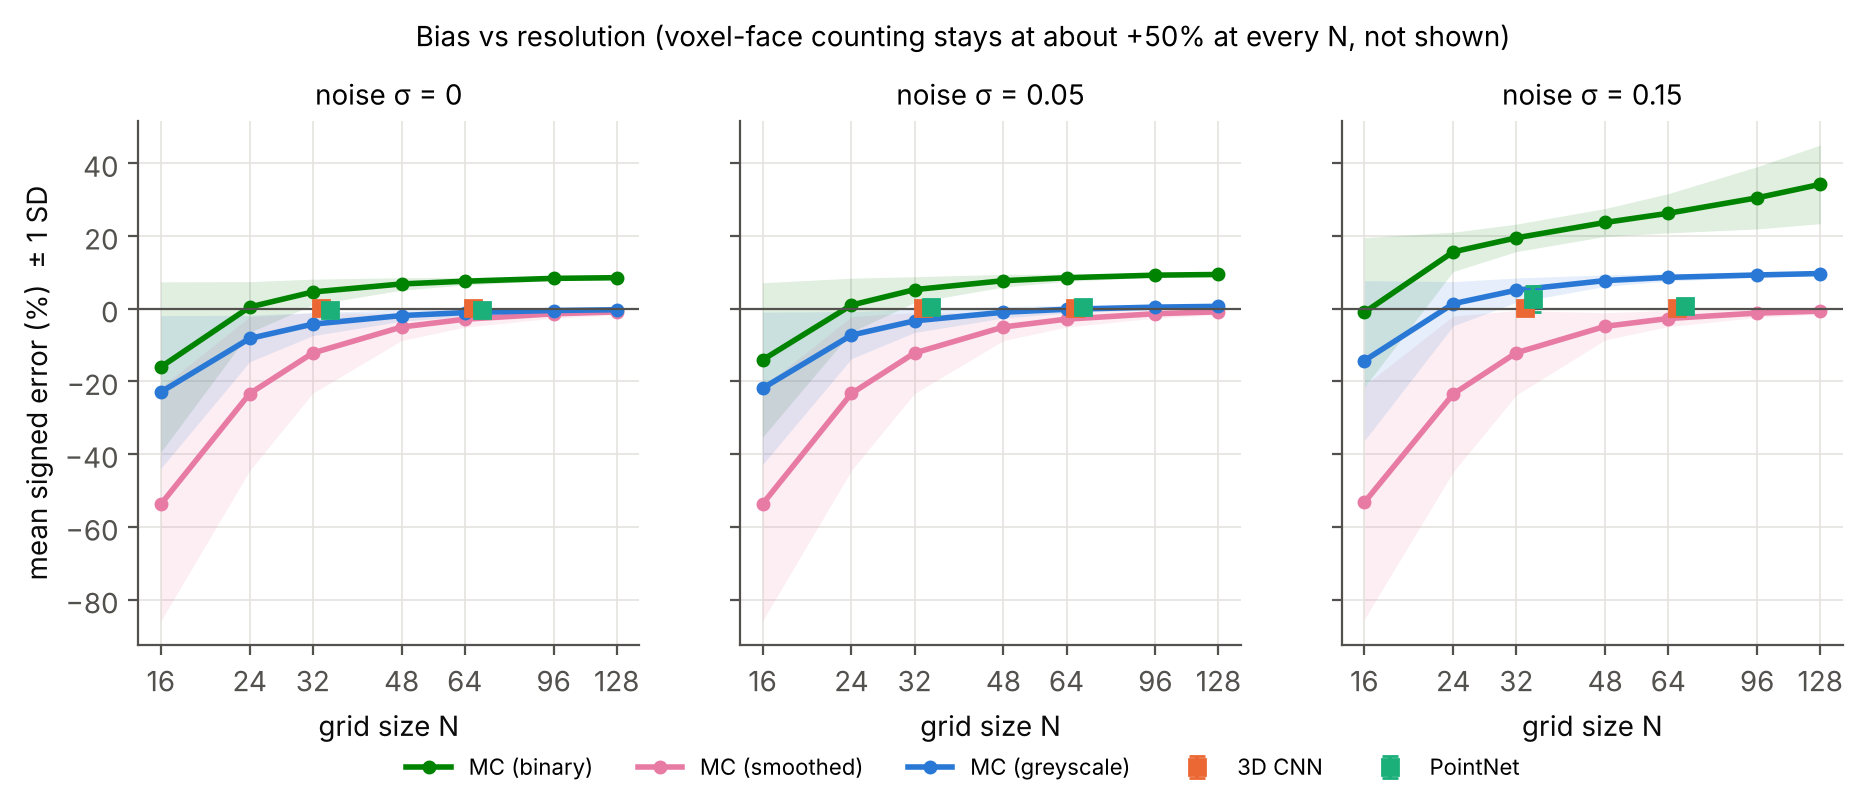
\includegraphics[width=0.86\textwidth]{bias_vs_resolution.png}
  \begin{itemize}\small
    \item Binary MC: clean $+0.5\% \to +8.5\%$ from $24^3$ to $128^3$; with noise $+16\% \to +34\%$.
    \item Greyscale MC: $-22.9\%$ at $16^3$ (curvature), $+9.7\%$ at $128^3$ with noise.
    \item Learned models (squares) stay near zero at the two sizes they were trained on.
  \end{itemize}
\end{frame}

% 34
\begin{frame}{Results: shape families never seen in training}
  \begin{columns}[T]
    \begin{column}{0.52\textwidth}
      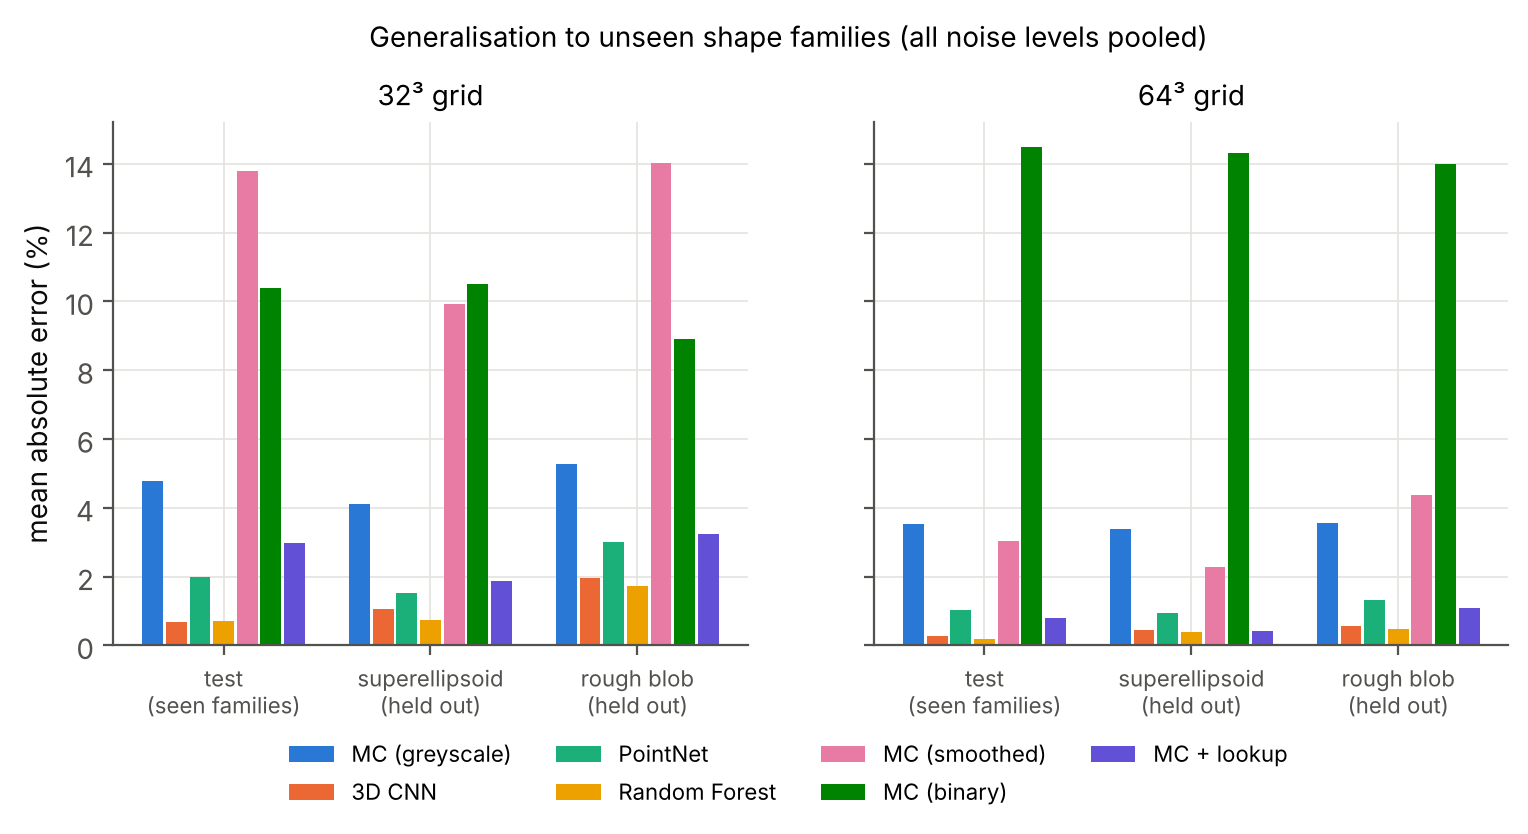
\includegraphics[width=\linewidth]{heldout_families.png}
    \end{column}
    \begin{column}{0.44\textwidth}
      \begin{itemize}
        \item \textbf{Superellipsoids} (sharp edges): CNN 1.05\% / 0.45\%, Random Forest 0.73\% /
              0.39\%, greyscale MC 4.10\% / 3.38\%.
        \item \textbf{Rough blobs}: hardest case, CNN 1.96\% / 0.55\%. Biased low: roughness
              smaller than a voxel is not in the image.
        \item Errors are 1.0 to 2.2 times the test-set errors: a moderate gap.
      \end{itemize}
    \end{column}
  \end{columns}
\end{frame}

% 35
\begin{frame}{Results: a failure case}
  \begin{itemize}
    \item The $32^3$ errors have a long tail: the CNN's average error is 0.68\%, but its spread is
          3.1\%.
    \item Most of that comes from one torus with a tube only \textbf{1.77 voxels} thick.
    \item After blurring, most of the tube never reaches the 0.5 level:
          greyscale MC finds only \textbf{42 of 142} units of area; the smoothed volume finds none.
    \item Every model is off by 47\% to 66\%.
  \end{itemize}
  \vspace{0.5em}
  \begin{alertblock}{Lesson}
    A correction can fix a biased surface, but not a surface that is missing from the mesh.
  \end{alertblock}
\end{frame}

\section{Conclusion}
% 36
\begin{frame}{Which method should you use?}
  \centering
  \begin{tabular}{p{4cm}p{8.5cm}}
    \toprule
    Situation & Recommendation \\
    \midrule
    Any case & Do not use voxel faces or binary MC for absolute area. \\
    Large, clean objects & Greyscale MC is already within about 1\%. \\
    Noisy scans & A learned correction brings the error to about 1\% or less. \\
    Objects under 16 voxels & Use the 3D CNN: 1.24\%, against 6.43\% for greyscale MC. \\
    Thinner than 2 voxels & No method tested here is reliable. \\
    \bottomrule
  \end{tabular}
\end{frame}

% 37
\begin{frame}{Conclusion}
  \begin{enumerate}
    \item The classical errors are not random: they come from geometry, curvature and noise, and
          simple theory predicts them.
    \item The best corrections reach 0.68\% ($32^3$) and 0.18\% ($64^3$) on unseen test shapes,
          from 4.78\% and 3.52\%.
    \item They still work on shape families never seen in training, with errors below 2\%.
    \item A simple Random Forest does as well as the 3D CNN in most cases.
  \end{enumerate}
\end{frame}

% 38
\begin{frame}{Limitations}
  \begin{itemize}
    \item \textbf{Simplified CT physics}: noise added to the image, not to the X-ray projections; no
          artefacts such as beam hardening or rings.
    \item \textbf{One object per volume}: real materials have many touching structures.
    \item \textbf{Fixed scan settings}: two grid sizes, three noise levels, fixed blur.
    \item \textbf{Sub-voxel detail}: on rough surfaces the correction is a learned guess, not a
          measurement.
    \item \textbf{Simple shapes, no tuning}: each model trained once; the $64^3$ CNN only 15 epochs.
    \item \textbf{No real scan} with a known surface area yet.
  \end{itemize}
\end{frame}

% 39
\begin{frame}{Next steps}
  \begin{enumerate}
    \item \textbf{Realistic CT simulation}: simulate the X-ray projections, Poisson noise and the
          reconstruction, instead of adding noise to the image.
    \item \textbf{Many objects per volume}: foams, porous rocks and printed lattices.
    \item \textbf{Real data}: scan an object whose surface area is known and check the correction.
    \item \textbf{More training}: longer training at $64^3$, and more shape types.
  \end{enumerate}
\end{frame}

% 40
\begin{frame}
  \centering
  \vspace{2em}
  {\Huge Thank you}\\[1.5em]
  Manas Jain \quad\textbar\quad 24123021
\end{frame}

\end{document}
